\section{Partialtonverläufe}
\label{sec:1}

\subsection{}
\texttt{loadRecordings()}

\subsection{}
Siehe Abbildung \ref{fig:ampl}.

\begin{figure}[H]
    \centering
    \begin{subfigure}{.5\textwidth}
        \centering
        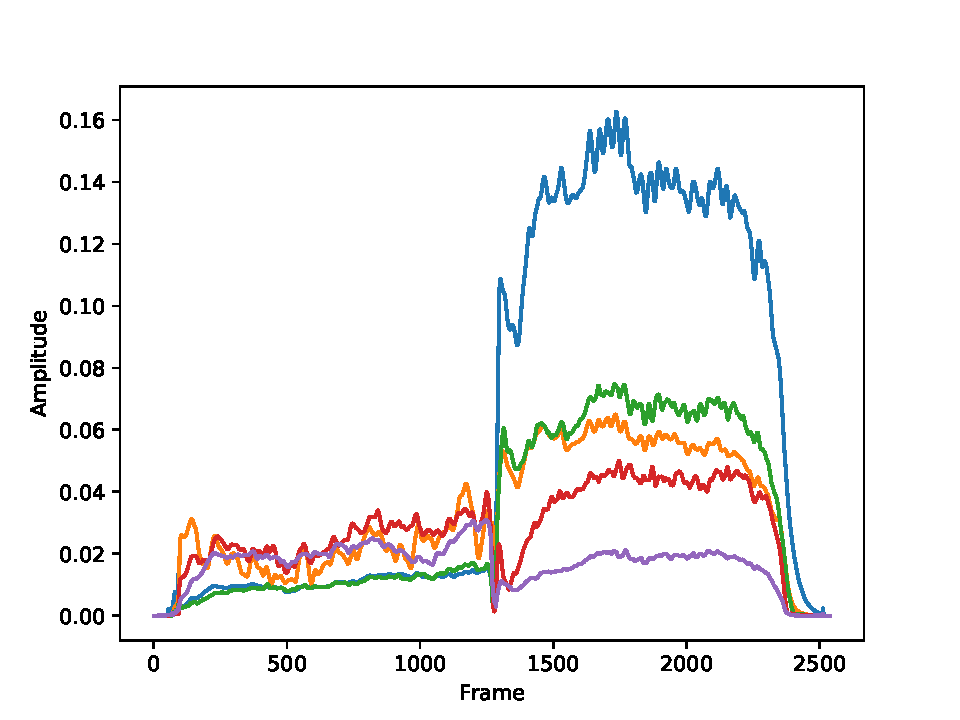
\includegraphics[width=\linewidth]{Figures/Buk04_amplitudes.pdf}
        \caption{BuK\_04}
        \label{fig:sub1}
    \end{subfigure}%
    \begin{subfigure}{.5\textwidth}
        \centering
        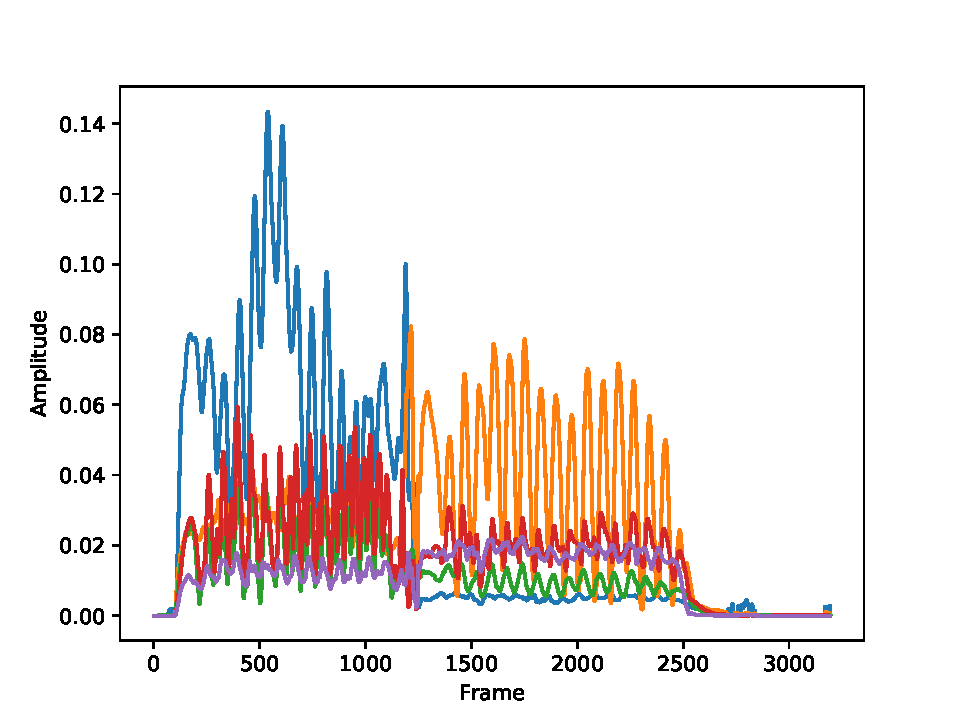
\includegraphics[width=\linewidth]{Figures/Buk23_amplitudes.pdf}
        \caption{BuK\_23}
        \label{fig:sub2}
    \end{subfigure}
    \caption{Amplitudenverlauf der ersten fünf Partialtöne}
    \label{fig:ampl}
\end{figure}

\subsection{}
Siehe Abbildung \ref{fig:freq}.

\begin{figure}[H]
    \centering
    \begin{subfigure}{.5\textwidth}
        \centering
        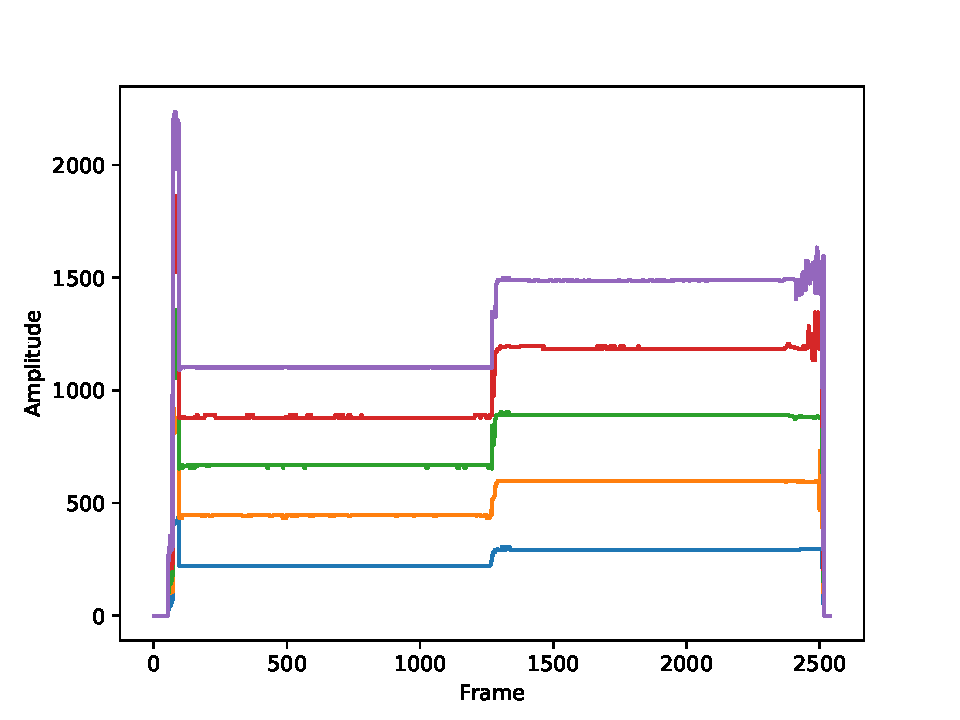
\includegraphics[width=\linewidth]{Figures/Buk04_frequencies.pdf}
        \caption{BuK\_04}
        \label{fig:sub1}
    \end{subfigure}%
    \begin{subfigure}{.5\textwidth}
        \centering
        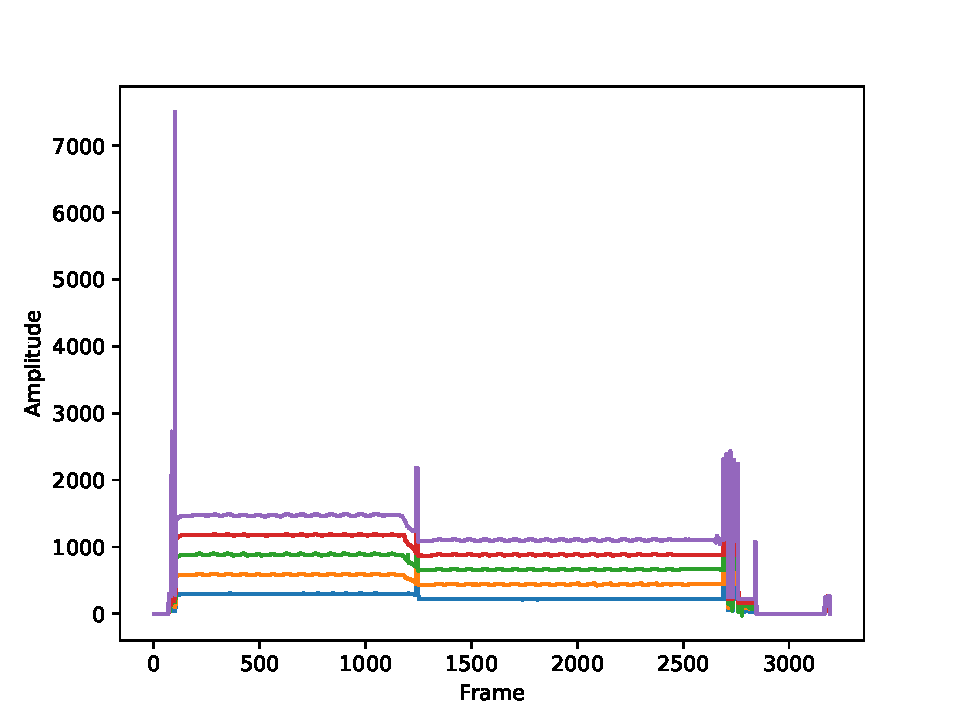
\includegraphics[width=\linewidth]{Figures/Buk23_frequencies.pdf}
        \caption{BuK\_23}
        \label{fig:sub2}
    \end{subfigure}
    \caption{Frequenzverlauf der ersten fünf Partialtöne}
    \label{fig:freq}
\end{figure}


\section{Strikte Harmonische Sysnthese}
\label{sec:2}

\subsection{}


\subsection{}


\section{Freie Harmonische Sysnthese}
\label{sec:3}

\subsection{}

\subsection{}


\section{Berücksuchtugung der originalen Phasen}
\label{sec:4}